\documentclass[12pt, a4paper]{article}
\usepackage[utf8]{inputenc}
\usepackage{amsmath}
\usepackage{amsfonts}
\usepackage{amsthm}
\usepackage{graphicx}
\usepackage{parskip}
\usepackage{hyperref}
\usepackage{fancyhdr}
\usepackage{lastpage}
\usepackage{tikz}
\usepackage{float}
\usepackage{listings}
\usepackage{color}
\usepackage{caption}
\usepackage[acronym]{glossaries}
\usepackage[nottoc]{tocbibind}
\usepackage[cache=false]{minted}
\usemintedstyle{default}
\newminted{haskell}{frame=lines,framerule=2pt}
\graphicspath{{./images/}}

\tikzstyle{bag} = [align=center]

\title{%
      Homework 3 \\
      Experimental Test of Ternary Search Tree Features
}
\author{%
  Juan Pablo Royo Sales \\
  \small{Universitat Politècnica de Catalunya}
}
\date\today

\pagestyle{fancy}
\fancyhf{}
\fancyhead[C]{}
\fancyhead[R]{Juan Pablo Royo Sales - UPC MIRI}
\fancyhead[L]{ADS - Homework 3}
\fancyfoot[L,C]{}
\fancyfoot[R]{Page \thepage{} of \pageref{LastPage}}
\setlength{\headheight}{15pt}
\renewcommand{\headrulewidth}{0.4pt}
\renewcommand{\footrulewidth}{0.4pt}

\newacronym{haskell}{Haskell}{Haskell Programming Language}
\newacronym{kde}{KDE}{Kernel Density Estimate}
\newacronym{lrm}{LRM}{Linear Regression Model}
\newacronym{tst}{TST}{Ternary Search Tree}
\newacronym{map}{HM}{Hash Map}
\newacronym{st}{ST}{Search Tries}
\newacronym{bst}{BST}{Binary Search Trees}

\begin{document}

\maketitle

\section{Introduction}\label{sec:intro}
In this work, I am going to try to reproduce the results exposed in this work \cite{cs_tst} that was proposed as a proper cover of \acrfull{tst} in the Lecture that we have about this topic.

As it is mentioned in the article \acrlong{tst} combine the best attributes of \acrfull{st} and \acrfull{bst}, in which it is stored a single character per letter like \acrshort{st} but in a \acrshort{bst} like structure with 3 nodes per level to improve space usage. In that sense they are very fast for searching as \acrshort{st} and efficient in space like \acrshort{bst}.

The experiments I have conducted are based on this \textbf{2(two)} main features of the Data Structure:

\begin{itemize}
  \item \textbf{Efficient in Running time}: For this experiment I have try to reproduce the same experiment as it is in the article doing an empirical comparison with \acrfull{map} Data Structure, which although it is $O(1)$ theoretically in searching, experimentally it needs to hash the \textbf{term} and the total time of the search is greater than the empirical time of searching on \acrshort{tst}.
  \item \textbf{Efficient in Space}: The same here we have compared space efficiency with \acrshort{map}.
\end{itemize}

\section{Asset organization}
Please check the appendix~\ref{apx:org} to see how the different assets are organized, how to run the experiment, and so on.

\section{Implementation}
\acrshort{tst} implementation in \acrfull{haskell} is really short and easy to read as we can see here:


\begin{listing}[H]
  \inputminted[firstline=16, lastline=56, breaklines]{haskell}{../src/Data/Tree/TST.hs}
  \caption{Extracted from source code src/Data/Tree/TST.hs}
  \label{src:tst}
\end{listing}


\section{Data Source}
The experiments that I have run are using the data under \mintinline{bash}{/usr/share/dict/words} which contains $235886$ dictionary words. For running the experiments I've divided the data in 2 data set:

\begin{itemize}
  \item $235886$ words for loading the whole structure.
  \item $117943$ words which is the half of the original data set, in order to search each of those words in the original data set.
\end{itemize}

\section{Experiments Details}
As I pointed out in the Introduction section~\ref{sec:intro}, I have defined 2(\textbf{two}) experiments.

\begin{itemize}
  \item \textbf{Benchmark Running Time}
  \item \textbf{Profile Space footprint}
\end{itemize}

The machine used to run the experiment is \textit{2,2 GHz 6-Core Intel Core i7} with \textit{32 Gb RAM}.

\subsection{Benchmark Running Time}\label{sub:sec:bench}
For the benchmarking I have used \cite{criterion} tool. Basically this library run several samples of the same process to take statistical analysis of the running time of the process. With that statistical information it builds a \acrfull{kde} graphic and a \acrfull{lrm}.

The benchmarking experiments are going to be focus on the following comparisons:

\begin{itemize}
  \item Running time of Searching $117943$ in \acrshort{tst} already loaded with $235886$ words
  \item Running time of Searching $117943$ in \acrshort{map} already loaded with $235886$ words
\end{itemize}

\subsection{Profile Space footprint}
For doing the profile space footprint analysis I have basically run the same experiments run on Benchmark but using the \acrshort{haskell} GHC profiling tools we can have the total amount of bytes allocated in GHC Garbage Collector for each structure.

Although this comparison is not one-to-one with a Digital Trie which would be the optimum, it is enough to see that I can show through this experiment that the structure allocates almost the same amount of of memory than \acrshort{map}.

\section{Results}
\subsection{Benchmark Running Time}
This are the graphics after running the benchmark analysis.

\begin{minipage}[t]{\linewidth}
  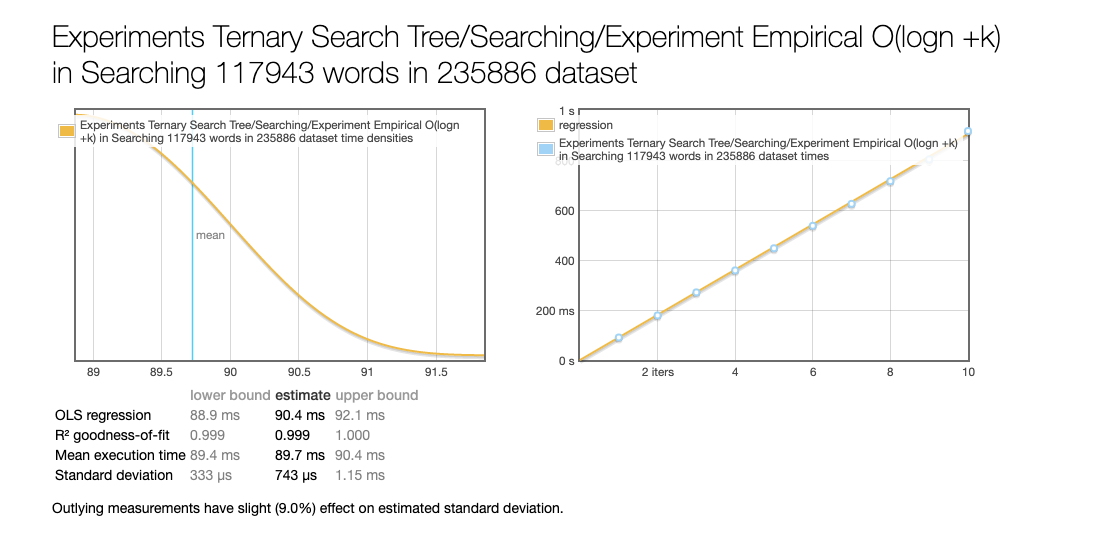
\includegraphics[width=\textwidth]{tst_bench}
  \captionsetup{type=figure}
  \captionof{figure}{TST Benchmark}
  \label{fig:tst_bench}
\end{minipage}

\begin{minipage}[t]{\linewidth}
  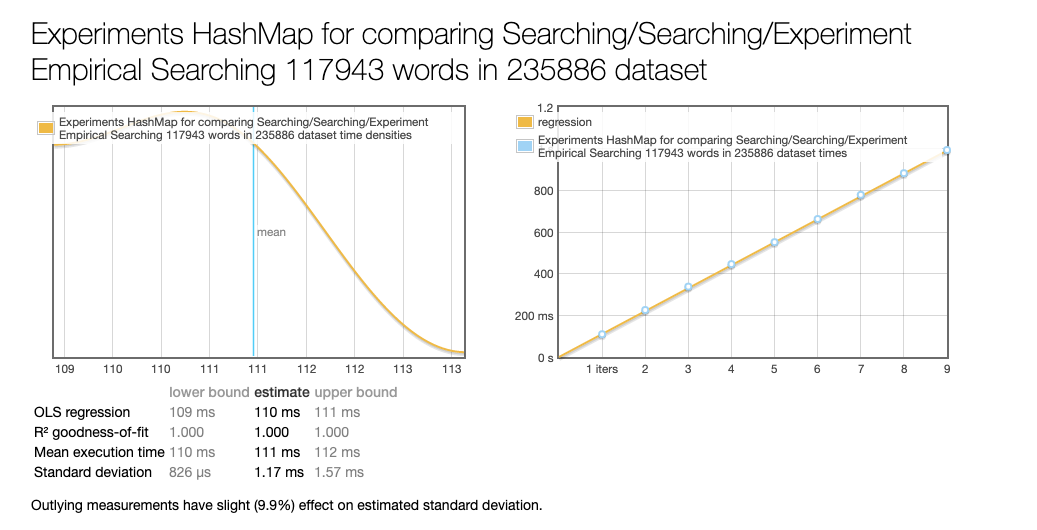
\includegraphics[width=\textwidth]{map_bench}
  \captionsetup{type=figure}
  \captionof{figure}{HashMap Benchmark}
  \label{fig:map_bench}
\end{minipage}

As we can see on the results \textbf{searching} in \acrshort{tst} has best performance than \acrshort{map} with a \textit{Mean Estimate time} of $89.7$ \textit{ms} compared with \acrshort{map} that is taking $111$.

If we compared this number with the number exposed in the article \cite{cs_tst}, having that the machine used at that time is much more slower than this one with a median of $520$ \textit{ms} it is obvious that the running comparison in terms of percentage is the same with a difference between 2 structures of $15\%$ less of running time in searching for \acrshort{tst}.

\subsection{Profile Space footprint}\label{sub:sec:qual:results}

\begin{minipage}[t]{\linewidth}
  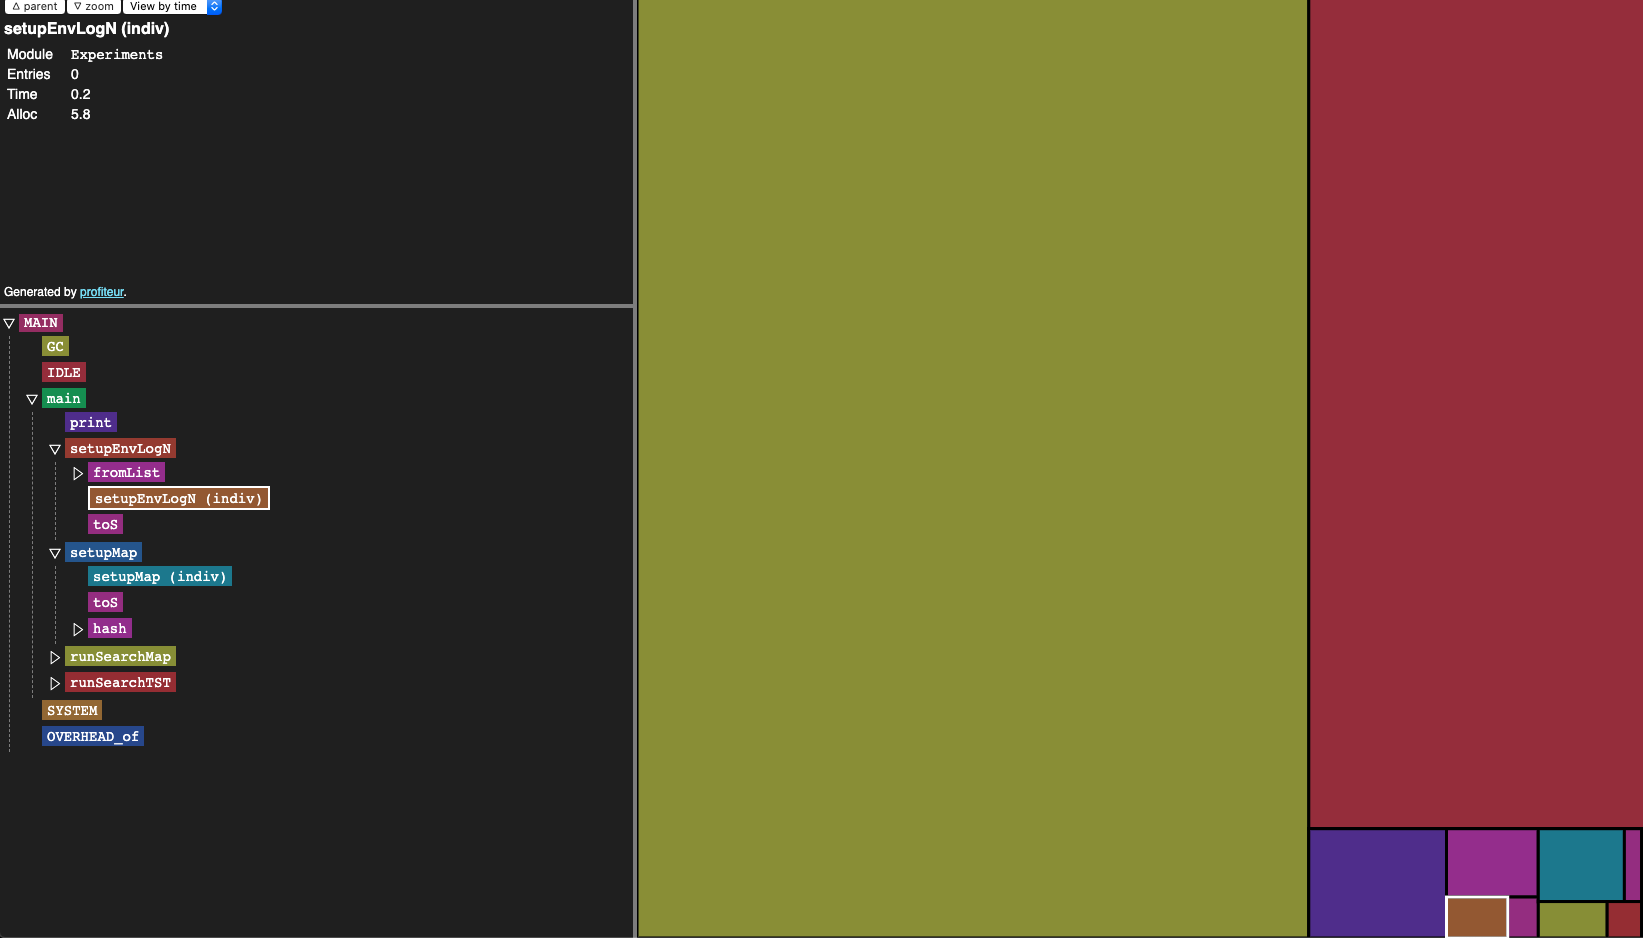
\includegraphics[width=\textwidth]{alloc_tst}
  \captionsetup{type=figure}
  \captionof{figure}{TST Memory footprint}
  \label{fig:alloc_tst}
\end{minipage}

\begin{minipage}[t]{\linewidth}
  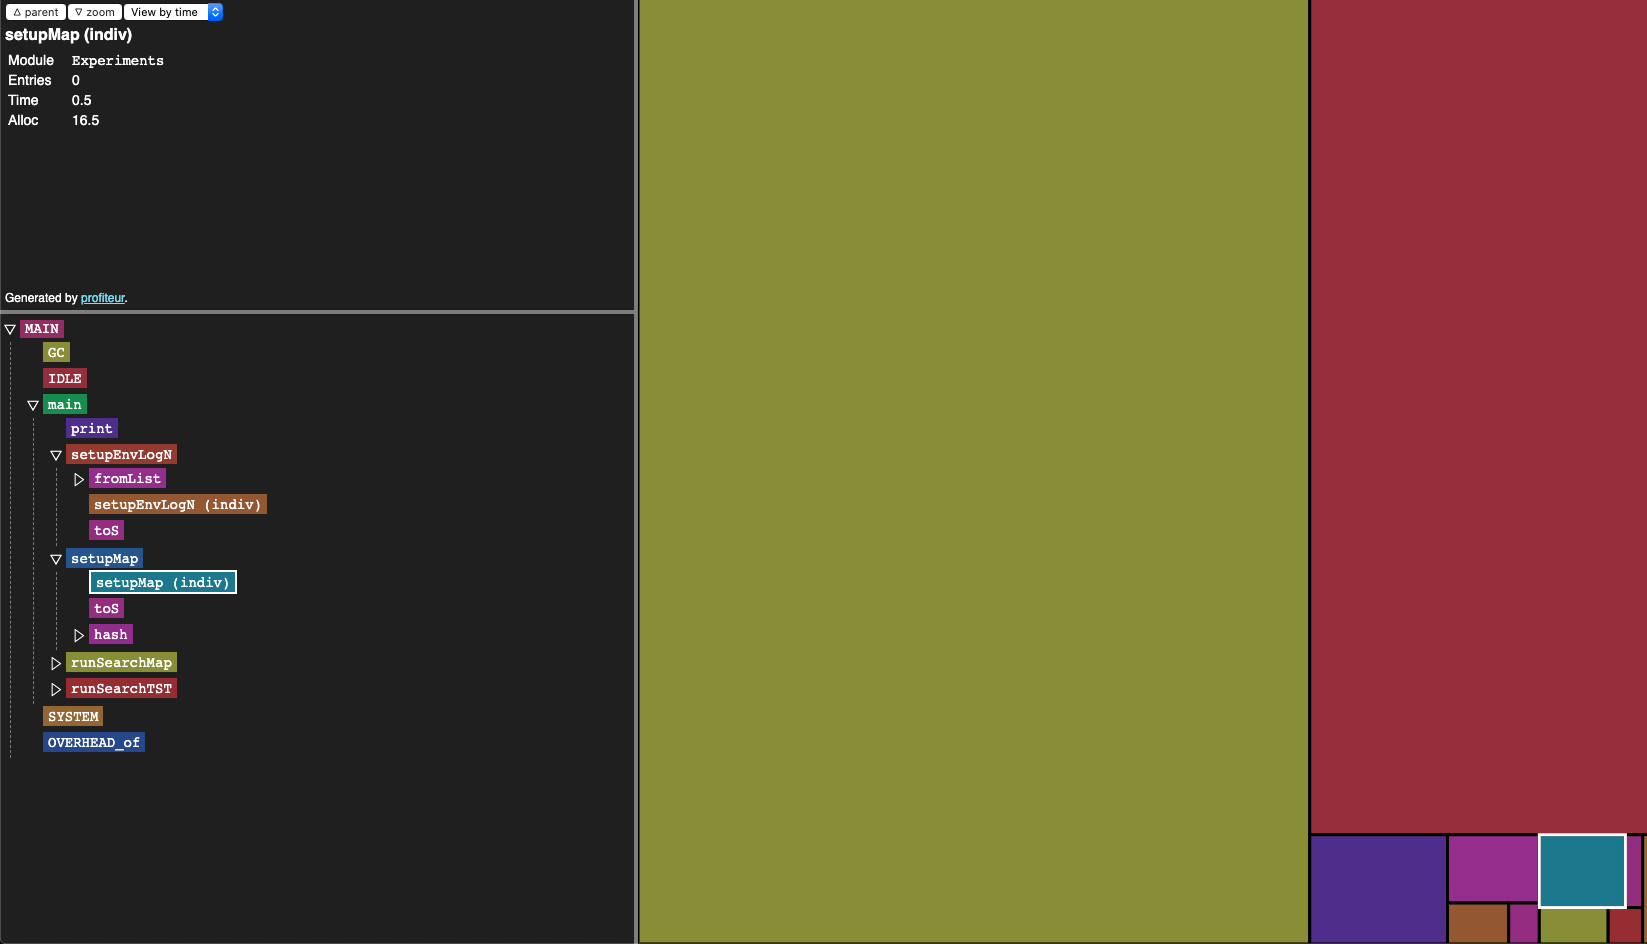
\includegraphics[width=\textwidth]{alloc_hash}
  \captionsetup{type=figure}
  \captionof{figure}{Map Memory footprint}
  \label{fig:alloc_map}
\end{minipage}

As we can see in the profiling experiment the amount of \textbf{Kb} allocated for \acrshort{tst} ($5.8 \text{Kb}$)  is less than \acrshort{map} ($16.5 \text{Kb}$) by a factor of 3, which is impressive.

\section{Conclusions}
In conclusion I was able to reproduce the experiments proposed in the article and shows experimentally that \acrfull{tst} is a running time and space efficient structure for dealing with String word searching.

On the other hand, one of the important thing of this Data Structure is that it is a really easy to implement structure and moreover taking the advantage of a Functional Programming language like Haskell that express Trees idiomatically better than an imperative counterpart.


\bibliographystyle{alpha}
\bibliography{report}

\printglossary[type=\acronymtype]

\appendix\label{apx:org}
\section{Haskell}
\subsection{Source Code}
In the source code there are 3 folders with code:

\begin{itemize}
  \item \textbf{app}: Which contains 2 programs with the 2 executables source code file. Here we can find:
    \begin{itemize}
      \item \textbf{\mintinline{haskell}{app/bench/Main.hs}}: It is the main entry point that run the Benchmark analysis in both Data Structures \acrshort{tst} and \acrshort{map}.
      \item \textbf{\mintinline{haskell}{app/profile/Main.hs}}: It is the main entry point that runs a profiling memory footprint to see what Data Structure occupies more space.
    \end{itemize}
  \item \textbf{src}: Contains the implementation source code of \acrshort{tst}.
    \begin{itemize}
      \item \textbf{\mintinline{haskell}{src/Experiments.hs}}: It contains the different experiment run.
      \item \textbf{\mintinline{haskell}{src/Data/Tree/TST.hs}}: \acrshort{tst} Implementation.
    \end{itemize}
  \item \textbf{test}: Contains Property based testing that automatize the test of the implemented \acrshort{tst}
\end{itemize}

\subsection{Run the Code}
All the solution has been coded with \textbf{Stack} \cite{stack} version 2.1.3 or higher. It is a prerequisite to install \textit{stack} for running this code.

\subsubsection{Running Experiments}
In order to run the experiments just do the following in each case.

\begin{itemize}
  \item \textbf{Benchmark Experiment}

\begin{minted}{bash}
stack build
stack exec tst-bench -- --output MY_OUTPUT_FILE.html
\end{minted}

This is going to left an HTML report with the benchmark results in \mintinline{bash}{MY_OUTPUT_FILE.html}

\item \textbf{Profiling Experiment}

\begin{minted}{bash}
stack build --profile
stack exec --profile tst-profile --  +RTS -pa -h
profiteur tst-profile.prof
\end{minted}

This is going to left an HTML report with the benchmark results in \mintinline{bash}{tst-profile.prof.html}

\end{itemize}

\section{Data Source - Input}\label{apx:data}
Input data or Data Source is being store under \mintinline{haskell}{data} folder.

\section{Generated Outputs}\label{apx:reports}
All the Generated Outputs that has been used to build this document are under \mintinline{haskell}{output} folder.

\section{Report PDF Document}
This report document is under \mintinline{haskell}{doc} folder alongside images that are embedded in this report.

\end{document}

